\chapter{Krav}
I starten af projektet var der opstillet nogle krav til produktet. Vores system skulle være i stand til at indsamle EKG-data, detektere en selvvalgt hjertesygdom og lagre abnormale EKG i en database. Disse krav ligger til grund for de tre væsentligste Use Cases (se figur.....)

\begin{figure}[htb]
	\centering
	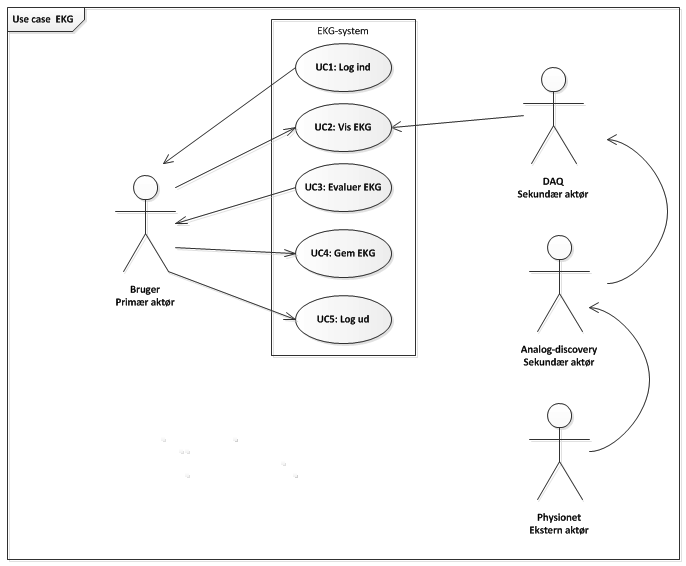
\includegraphics[width=1\textwidth]{Figurer/Snip20150518_11}
	\caption{Use case-diagram}
	\label{fig:Use Cases}
\end{figure}

Som vist på figuren, er der i alt 5 Use Cases som beskriver, systemets funktionelle krav. De vigtigste Use Cases er UC2, UC3 og UC4, da de nævnt tidligere er i forvejen opstilte krav til projektet. Inden programmet kan startes er der dog tilføjet visse krav til anvendelse. Hver bruger skal have et personligt login, så de på den måde "underskriver" målingerne, de foretager. Det gør det nemmere at rette henvendelse i tilfælde af spørgsmål til enkelte målinger. Desuden skal patientens CPR-nummer intastes.
Når EKG'et evalueres er programmet indstillet til at detektere sygdommen atrieflimmer. Hvis denne arytmi opstår på de målte EKG'er, meldes dette til brugeren af systemet. Dermed ved lægen, at der skal holdes øje med denne sygdom.
Når EKG-målinger gemmes vil de blive gemt i en SQL- og offentlig databse. Desuden gemmes de i forbindelse med patientens CPR-nummer. Dermed gøres det nemmere for sundhedsfaglig personale at finde den enkelte patients målinger.
De ikke-funktionelle krav er beskrevet udfra (F)URPS+ og MoSCOW metoden. Her beskrives hvilke krav der -stilles til systemts interface og pålidelighed.
For yderligere beskrivelse af både funktionelle og ikke-funktionelle krav se under 'Kravspecifikation' i projektdokumentationen.\\
Projektets produkt er en prototype. 